\documentclass[12pt]{article}
% --- 1. Core Layout & Formatting ---
\usepackage[utf8]{inputenc}
\usepackage[T1]{fontenc}
\usepackage{geometry}
\geometry{margin=1in}
\usepackage{setspace} 
\usepackage{titlesec}
\usepackage{bm}         % For bold math symbols (\boldsymbol)
\usepackage{amsmath, amssymb} % Math essentials

% --- 2. Graphics & Plotting ---
\usepackage{graphicx}
\usepackage{caption}
\usepackage{float}
\usepackage{tikz}
\usepackage{pgfplots}
\pgfplotsset{compat=1.18}

% --- 3. Tables ---
\usepackage{booktabs}
\usepackage{longtable}
\usepackage{tabularx}

% --- 4. TColorBox (The Boxed Text) ---
\usepackage[most]{tcolorbox}

% --- 5. Referencing ---
\usepackage{url}
\usepackage{hyperref} % This makes the DOI text an actual clickable link

% Define the "summarybox" environment
\newtcolorbox{summarybox}[2][]{%
  enhanced,
  drop shadow={black!50!white},
  coltitle=black,
  top=0.3in,
  attach boxed title to top left={xshift=1.5em,yshift=-\tcboxedtitleheight/2},
  boxed title style={size=small,colback=pink},
  title={\bfseries #2}, 
  #1
}

% Define the "Summary" theorem style (if you want numbered summaries)
\newtcbtheorem{Summary}{Summary}{
  enhanced,
  drop shadow={black!50!white},
  coltitle=black,
  top=0.3in,
  attach boxed title to top left={xshift=1.5em,yshift=-\tcboxedtitleheight/2},
  boxed title style={size=small,colback=pink}
}{sum}

% --- 5. Bibliography ---
\usepackage[style=numeric, sorting=none, backend=biber]{biblatex} 
% Ensure this file exists in your folder!
\addbibresource{bibliography_CIBB_file.bib}

% --- 6. Document Settings ---
\setlength{\parindent}{0pt}   
\setlength{\parskip}{1em}     

\captionsetup[figure]{
    format=hang,
    labelsep=quad,
    labelfont=bf,
    skip=15pt 
}

\title{Self-Evaluation Report \\ \large Computational Fracture Mechanics (WiSe26)}
\author{Bagus Alifah Hasyim \\ 108023246468}
\date{}

\begin{document}
\maketitle

\section*{Phenomenology of Fracture}

\section{Linear Elastic Fracture Mechanics (LEFM)}

\hspace{1em} As referring to the lecture, linear elastic fracture mechanics is a scope of fracture studies by means the crack consideration as a static crack, 
which implies no further investigation of crack propagation. The naming is also quite clear that LEFM mainly concern only on the elastic strain energy to the
fracture propagation, which is derived from the Griffith Fracture Criterion (GFC). The criterion states that fracture propagation is started as the decrease 
of the elastic strain energy of the material is equal to the increase in the surface energy of the fracture~\cite{Guo.2021}. To understand the relation of the
surface energy and the elastic strain energy, further illustration is shown in figure~\ref{fig:Energy}.

\hspace{1em} Consider an infinite plate with crack length of 2a that is subjected to a stress $\sigma$. 
The change of elastic energy $W_{el}$ and the surface energy $W_s$ are defined respectively as follows:

\begin{equation}
  W_{el} = -\frac{\pi \sigma^2 a^2}{E}; \space \space W_{s} = 4a \gamma_s 
  \label{eq:ElasticEnergy}
\end{equation}

Where $a$ is the crack length and $E$ is the young modulus. Notice that the minus sign is stated due to the fact that these phenomena is a decrease of elastic energy.
$\gamma_s$ is the surface energy of the crack, which increase as the crack length increase as well. Hence, Griffith postulation mentioned that 
a crack will extend if the potential energy decrease~\cite{Janssen.2002}. Potential energy is defined as the sum of the surface energy and the elastic energy, which is written as follows:

\begin{equation}
  U = W_s + W_{el}
  \label{eq:TotalEnergy}
\end{equation}

Therefore, the Griffith postulation can be written mathematically as follows:

\begin{equation}
  F_{crack} = -\frac{dU}{da} > 0
  \label{eq:Crack}
\end{equation}

From this relation, this can be explained that the negative quadratic term for the elastic energy decrease eventually the
contribution of the surface crack energy, which at some point the total energy curve is decreased. This turning point is considered
as the crack initiation criterion, which the slope begin to change to negative sign. 

\begin{figure}[H]
    \centering
    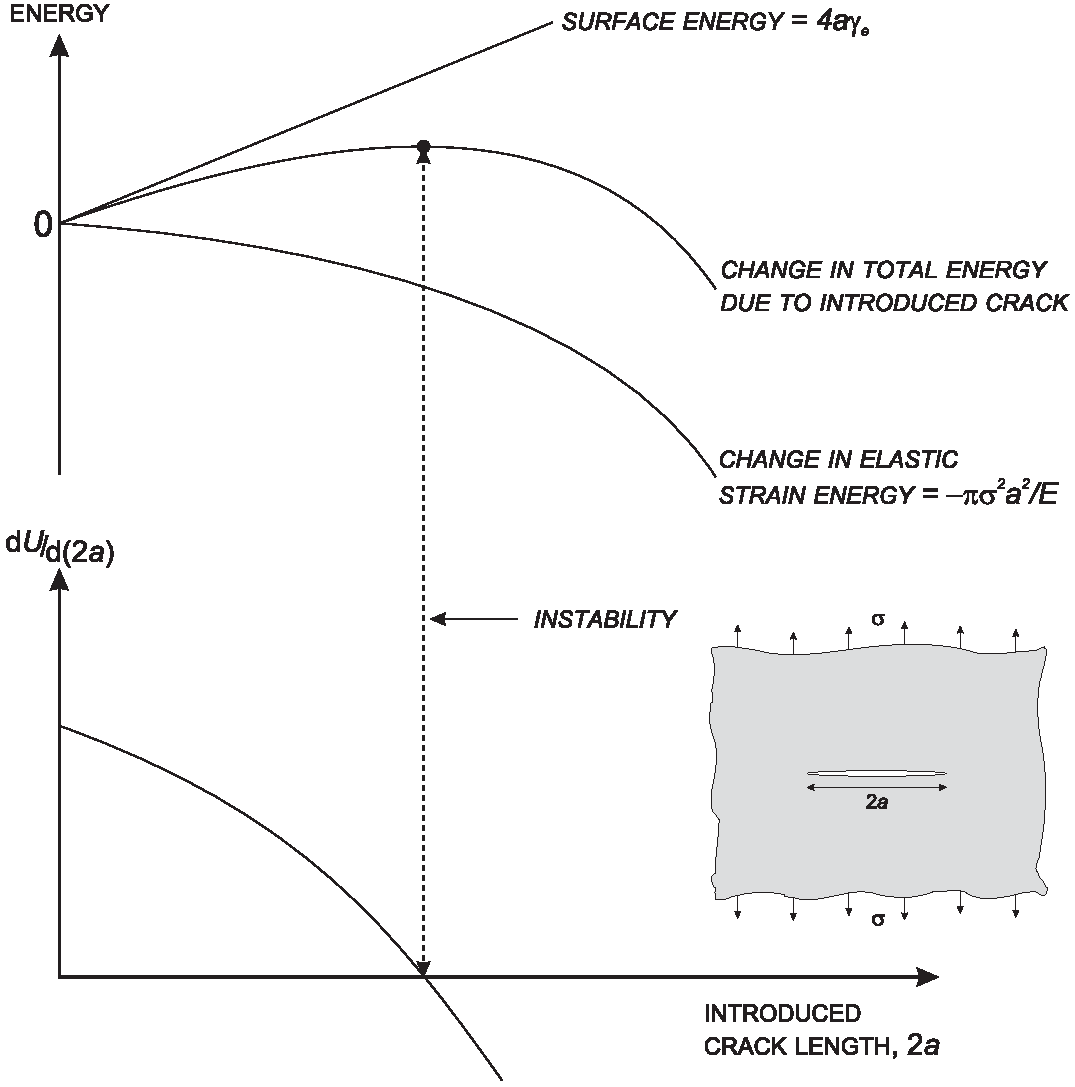
\includegraphics[width=0.5\textwidth]{images/Q1_Energy.pdf}
    \caption{Energy balance for small crack in a large plate loaded with fixed grip conditions~\cite{Janssen.2002}.}
    \label{fig:Energy}
\end{figure}

\hspace{1em} The energy/griffith method is considered impractical to apply in studying crack. Going by this Background, Irwin developed so call stress intensity approach in the 1950s. This
method basically utilized an additional dimensionless parameter K, which used to determine the stresses in the vicinity of the crack. The nomenclature in figure~\ref{fig:Stress} shows the calculated
stress determined from the tip of the crack which defined as follows:

\begin{equation}
  \sigma_{ij} = \frac{K_{I}}{\sqrt{2\pi r }} f_{ij}^{(I)}(\theta) + \frac{K_{II}}{\sqrt{2\pi r }} f_{ij}^{(II)}(\theta) + \frac{K_{III}}{\sqrt{2\pi r }} f_{ij}^{(III)}(\theta)
  \label{eq:Stress}
\end{equation}

\hspace{1em} Where $K$ is the stress intensity factor and $f_{ij}$ is a geometry factor, ranging a different equation or value for every different loading mode, crack dimension, crack position, and specimen dimension. The $ij$ subscript 
is defined for different stress state, for example $\sigma_{22}$ is used to describe the stress in the y-coordinates (for Cartesian coordinate usage). It can be inferred 
from equation~\ref{eq:Stress} that the stress will produce singularity at crack tip, knowing the $\frac{1}{\sqrt{r}}$ relation which can produces high stress concentration value. Noted that $f_{ij}$ and $K$ is dependent
on some certain of three modes or also known as how does the loading movement act on the crack. Therefore, equation~\ref{eq:Stress} is dependent on how does the loading act on the specimen with crack itself.
Single loading type, for example a simple tensile load in the crack specimen will leave only the $\frac{K_{I}}{\sqrt{2\pi r }} f_{ij}^{(I)}(\theta)$ term in the stress equation. Figure~\ref{fig:Mode} shows the typical mode that exist for such
specimen with crack.

\begin{figure}[H]
    \centering
    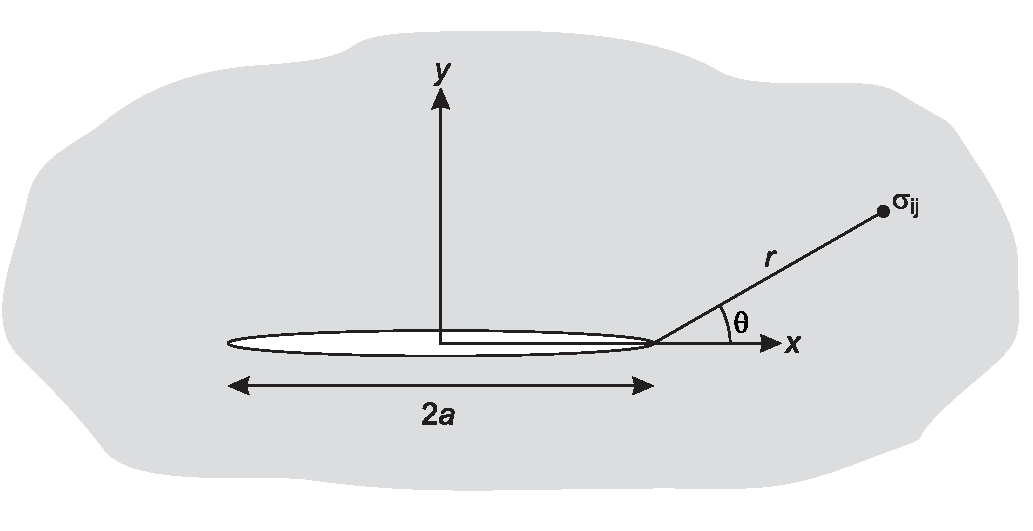
\includegraphics[width=0.5\textwidth]{images/Q1_StressCalc.pdf}
    \caption{Stresses at point tip with respect to the crack tip using polar coordinate~\cite{Janssen.2002}.}
    \label{fig:Stress}
\end{figure}

\hspace{1em}As mentioned in the beginning of this subchapter, LEFM have limitation only usage in a static crack and for brittle material. This is also due to the fact that
brittle material does not undergo extensive plastic deformation compared to the ductile material. Hence, the flow curve until failure can be evaluated
using LEFM approach.

\begin{figure}[H]
    \centering
    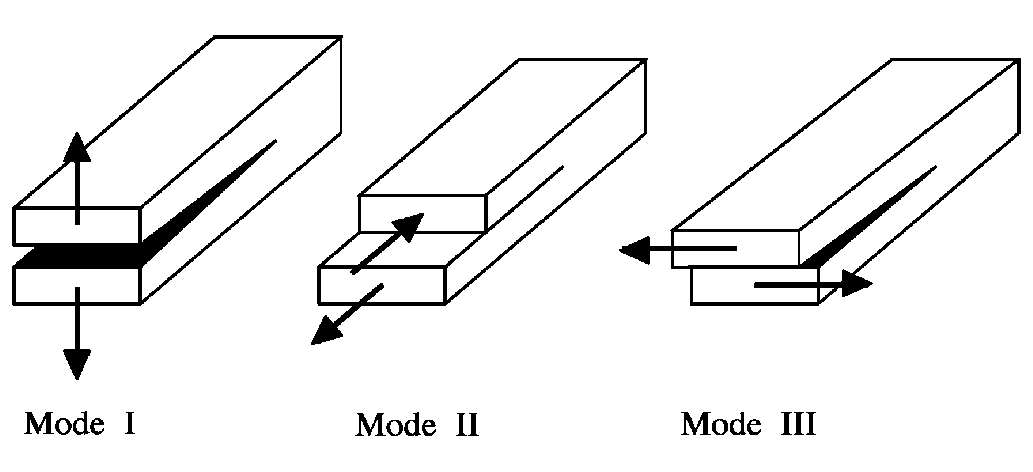
\includegraphics[width=0.55\textwidth]{images/Q1_Mode.pdf}
    \caption{Different type of loading mode (Mode I: Opening, Mode II: In-Plane Shear, Mode III: Out-of-Plane Shear)~\cite{Chang.2002}}
    \label{fig:Mode}
\end{figure}


\section{Elastic-Plastic Fracture Mechanics}

\hspace{1em} As discussed previously, linear elastic fracture mechanics have limitation on describing the fracture in the elastic region only. Beside known from the
naming, LEFM is limited to describe the behavior only for either plane strain fracture in very high strength metallic material or for brittle material such as glass, 
ceramics, rocks, and ice. Hence, elastic-plastic fracture mechanics (EPFM) is introduced to cover the area beyond the plastic region~\cite{Janssen.2002}.

\hspace{1em} EPFM have coverages in materials that exhibit time-independent with non-linear behavior. This requires additional parameterization to describe such behavior: The first
one is crack tip opening displacement (CTOD) and the J contour integral. Both of these parameters can describe the material in the elastic-plastic region and have the possibility for failure criterion utilization. Hence, 
CTOD and J integrals give a nearly size-independent fracture toughness measurement~\cite{Anderson.1995}.

\section{Failure hypotheses}

\subsection*{Critical Stress Intensity Factor}
\hspace{1em}As stated regarding the calculated stress in equation~\ref{eq:Stress}, K is mentioned as the stress intensity factor. K is basically a magnitude that gives elastic stress field.
Based on the dimensional analysis, K should be linearly related to the stress and directly related to the square root of a
characteristic length~\cite{Janssen.2002}. Hence, the equation is described as follows:

\begin{equation}
    K = \sigma \sqrt{\pi a} f(\frac{a}{w})
    \label{eq:SIF}
\end{equation}

Where $a$ is the crack length, $\sigma$ is the applied stress, and $f(\frac{a}{w})$ is a dimensionless parameter that depends 
on the specimen and crack. Based on the griffith energy balance approach on the crack initiation criterion, it is mentioned that crack is initiated in a certain condition, which written as follows:

\begin{equation}
    \sigma \sqrt{a} > \sqrt{\frac{2 E \gamma_e}{\pi}} 
    \label{eq:Criterion}
\end{equation}

Where $E$ and $\gamma_e$ are the material properties. Hence, the crack will initiate if such condition in equation~\ref{eq:Criterion} is met. The fulfillment of such condition
can be known as well as the critical stress intensity factor ($K_{IC}$), as this parameter describe the fracture toughness of the material or the material resistance against fracture~\cite{Zhu.2012}.   

\subsection*{Critical Energy Release Rate}
\hspace{1em} From Griffith theory, Irwin proposed a modification on the original crack extension criterion, where the equation is written as follows:

\begin{equation}
    \frac{\pi \sigma^2 a}{E} > 2 \gamma_e 
    \label{eq:Griffith}
\end{equation}

Where the proposal was made on the left-hand side modification, which it is defined as the energy release rate $G$. This term represented
the energy calculated per unit new crack area, available for infinitesimal crack extension~\cite{Janssen.2002}. While the right hand-side described the
surface energy increase per unit new crack area that would occur as well in infinitesimal crack extension. Irwin's modification can be written
as follows.

\begin{equation}
    G = \frac{\pi \sigma^2 a}{E} > G_c = 2 \gamma_e 
    \label{eq:Irwin}
\end{equation}

Using both of the solution from Griffith and Irwin's modification, a simple relation can be established between factor K and the energy release rate.

\begin{equation}
    \frac{K}{E'} = G
\end{equation}

Where $E' = E$ represent for plane stress condition, and $E' = E(1-\nu)$ for plane strain condition with $E$ represent young's modulus and $\nu$ is the Poisson's ratio~\cite{Zhu.2012}.
\subsection*{J-Integral}
\hspace{1em} To map the fracture behavior based on the work done on a material per area of fracture, J integral offers a method to evaluate the toughness
that exhibit non-linear behavior during loading~\cite{Hosford.2010}. It is proposed by Rice, as he formulated J integral to be a path independent line integral 
that extend from the crack tip, which then the potential energy is calculated per increment of the line. Hence, the value is decrease as the line integral extend out of the
crack tip~\cite{Janssen.2002}. Mathematically, J2 comes from the derivation of the second invariant of the deviatoric stress tensor, which defined as follows:

\begin{equation}
    J_2 = \frac{1}{2}(S_{ij}S_{ij})
    \label{eq:J2}
\end{equation}

Where $S_{ij}$ is the deviatoric stress component. As defined previously, the J integral is basically sum of the work done in such
path independent line integral. Here, it defines as following equation.

\begin{equation}
    J = \int_{}^{} W dy - T_{i}\frac{\partial u_i}{\partial x}s   
    \label{eq:J2}
\end{equation}

In other literature, the derivation begins from limit approach~\cite{Janssen.2002}. It is said that the decrease of potential energy
per increment of crack growth $-\frac{dU_p}{da}$, where the potential energy can be expressed as following terms.

\begin{equation}
    -\frac{dU_{\text{p}}}{da} = \lim_{\Delta a \to 0} -\frac{\Delta U_{\text{p}}}{\Delta a} = \lim_{\Delta a \to 0} \frac{1}{\Delta a} \left( \int_{\Gamma^*} T_i \Delta U_i \, ds - \int_{A^*} \Delta W \, dA \right).
    \label{eq:PotentialEnergy}
\end{equation}

Equation~\ref{eq:PotentialEnergy} can be visualized using following figure, as the sum of the potential energy is calculated
through the path perimeter $\varGamma$ with an area of $A$. Traction $T_i$ is subjected in the outer surface of the body $\varGamma*$,
which also the total perimeter that can be calculated.

\begin{figure}[H]
    \centering
    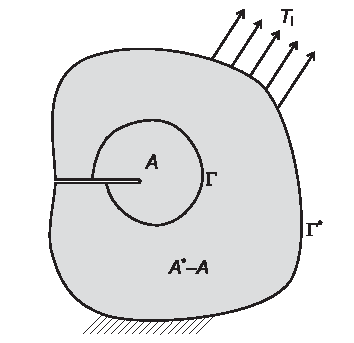
\includegraphics[width=0.65\textwidth]{images/Q3_JIntegral.pdf}
    \caption{Elastic body with arbitrary area of A defined with a crack tip~\cite{Janssen.2002}}
    \label{fig:JIntegral}
\end{figure}

\subsection*{Crack-Tip Opening Displacement}

\hspace{1em}Crack tip opening displacement (CTOD) is originated from the crack opening displacement
(COD) at the original crack tip, which is basically a study to measure the amount of plastic strain which
the specimen subjected to a displacement~\cite{Janssen.2002}. CTOD was proposed in 1963 by Wells to serve as an engineering fracture parameter,
equivalent to K or J in practical application~\cite{Zhu.2012}. Hence, the crack is study by measuring the crack blunt displacement near the crack tip after
the specimen subjected to a surface traction in the specimen.

\begin{figure}[H]
    \centering
    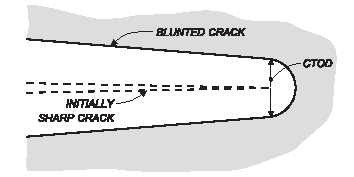
\includegraphics[width=0.45\textwidth]{images/Q3_CTOD.pdf}
    \caption{Crack tip opening displacement (CTOD) deformation from sharp to blunt crack~\cite{Janssen.2002}.}
    \label{fig:CTOD}
\end{figure}

\section{Crack resistance and R-curve behavior}
\hspace{1em}As mentioned in equation~\ref{eq:Irwin} in Irwin's modification, crack growth will initiate if the energy is larger than the critical energy release rate. Here according to the lecture, the critical
energy release rate is equal to the R-curve with function of crack length~\cite{Hartmaier.}. Hence, this study aim to examine the stability of the crack growth by comparing the crack resistance
$R(a)$ with the energy release rate. The crack resistance is defined as the energy required per increment of crack extension~\cite{Janssen.2002}. Thus, combining the energy release rate and crack resistance concept produce
following criterion of crack growth stability.

\begin{equation}
    \frac{\partial G}{\partial a}| _{F = const} \leq \frac{dR}{da} 
    \label{eq:RCurve}
\end{equation}

\hspace{1em}This crack growth stability example is shown in figure~\ref{fig:RCurve}. It is observed that two different R-Curves has their own behavior according to its crack-length-R relation. Hence, R is equivalent to the
applied force, which the value is growing exponentially as it tends to reach instability for larger R value. Hence, the critical G are present in both intersection point of the G- and R-Curve, where the derivative of both curves is equal.


\begin{figure}[H]
    \centering
    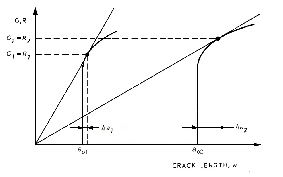
\includegraphics[width=0.48\textwidth]{images/Q3_RCurve.pdf}
    \caption{R-Curves and two example points of instability~\cite{Janssen.2002}.}
    \label{fig:RCurve}
\end{figure}


\newpage
\section*{Finite Element Modeling of Dynamic Cracks and Damage}
\section{Cohesive Zone Models}
\hspace{1em} In finite element method concept, there are two main restrictions that should be taken account in introducing crack. The first one is the restriction of displacement jump
as in FEM the connected element should have at least follows $C^0$ continuity. The second restriction is that stress should fulfill mesh dependency, meaning that the generated stress is influence
 by the difference of mesh sizes and shape type~\cite{Hartmaier.}. To address the first restriction, cohesive zone method is introduced.

\hspace{1em} Cohesive zone method (CZM) is a notably known method use to introduce crack in finite element analysis, which additional element so call cohesive material or glue is defined in between
two elements. This implied to the state that the crack can only grow through the defined cohesive element, restricting random crack propagation direction. In this model, additional constitutive relation so call traction-separation law is introduced 
as the cohesive element material.

\begin{figure}[H]
    \centering
    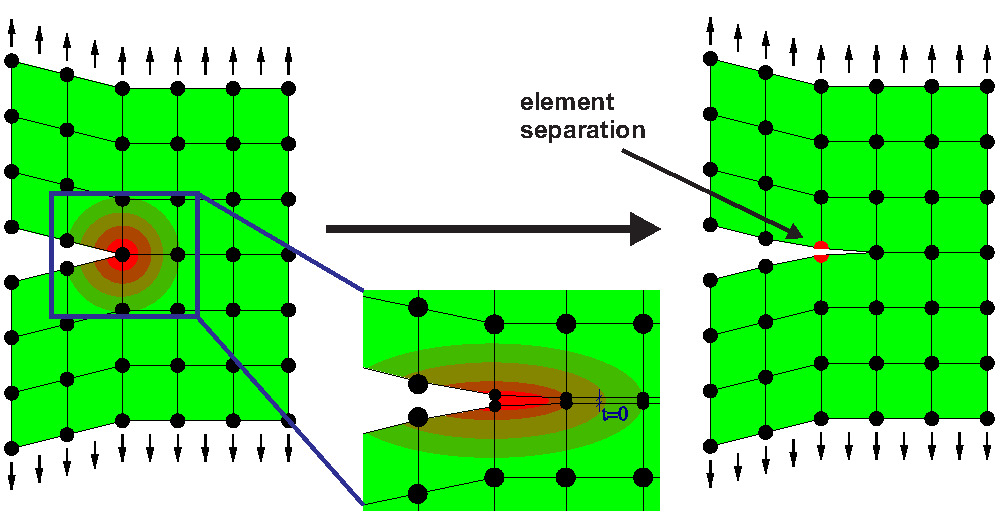
\includegraphics[width=0.6\textwidth]{images/Q5_CohesiveElement.pdf}
    \caption{Cohesive zone method mechanism with the zoomed in point of view on the traction criterion~\cite{Hartmaier.}}
    \label{fig:Cohesive}
\end{figure}

\hspace{1em} To understand the CZM, figure~\ref{fig:Cohesive} shows the mechanism of the separation for side crack in a finite plate specimen with tensile load on both direction. As the displacement increase over time,
stress concentration is accumulated in the crack tip. The stress will eventually exceed the criterion, which here is the defined stress threshold for the cohesive element. The element will separate as this criterion is fulfilled,
moving the crack tip further to the deeper cohesive element, which then it will continue to propagate until the end of the defined cohesive element. As shown in figure~\ref{fig:Stress}, the crack is highly dependent on the mesh
size and shape, which is correlated to the defined cohesive element. 

\hspace{1em} The constitutive equation of CZM, which mentioned previously, use the traction-separation law. 
Here, the law is defined through traction-displacement curve in figure~\ref{fig:TractionSeparation}. The curve show relation of stress or traction, denote as T and separation marked as
$\delta$. The stiffness $E_0$ is defined so that the critical displacement $\delta_C$ is defined, with the traction threshold T as well. If the displacement and traction reach the maximum
peak, the cohesive element starts to undergo strain-softening, decrease in stiffness and eventually leads to complete separation in a prescribed
displacement of $\delta_f$. The area below curve, denote as $G_c$ is known as fracture energy, which the area is equivalent to the triangle area for this case. This implies the minimum energy in which fracture or
separation is initiated, in other words.

\begin{figure}[H]
    \centering
    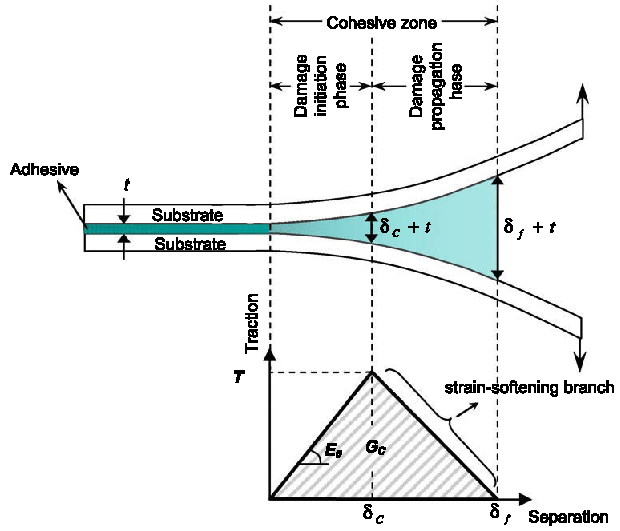
\includegraphics[width=0.6\textwidth]{images/Q5_TractionSeparation.pdf}
    \caption{Traction-separation curve visualized in the two plates separation~\cite{Khoramishad.2010}.}
    \label{fig:TractionSeparation}
\end{figure}

\section{Extended Finite Element Method (XFEM)}
\hspace{1em}On previous chapter, the restrictions in FEM are discussed, especially the strictness of minimum $C^0$ continuity to fulfill conformity of the mesh. Introducing
extended finite element method (XFEM), where this approach couples the conventional conform displacement and allowing displacement jump, representing the crack propagation.
The element is enriched with additional boundary $\varGamma_{crack}$, separating the body into $\Omega^+$ and $\Omega^-$~\cite{Hartmaier.}. Hence, the strain can be defined using two terms as following.

\begin{equation}
  \varepsilon(x,t) = \nabla u_{conv} (x,t) + H(x) \nabla u_X (x,t)  
  \label{eq:Strain}
\end{equation}

\hspace{1em}Where $H(x)$ is a jump function, distinguishing the $\Omega^+$ and $\Omega^-$~\cite{Hartmaier.}. Hence, XFEM is basically an enriched element which have additional stiffness for the crack or the displacement jump. As a visualization, mathematically the
linear equation for XFEM that solve for such conventional and crack (jump) displacement is written as follows:

\begin{equation}
\begin{vmatrix}
\mathbf{K}_{\text{conv}} & \mathbf{K}_{\text{conv},X} \\
\mathbf{K}_{\text{conv},X}^T & \mathbf{K}_{X,X}
\end{vmatrix}
\begin{vmatrix}
\mathbf{u}_{\text{conv}} \\
\mathbf{u}_{X}
\end{vmatrix}
=
\begin{vmatrix}
\mathbf{f}_{\text{ext,conv}} \\
\mathbf{f}_{\text{ext},X}
\end{vmatrix}
-
\begin{vmatrix}
\mathbf{f}_{\text{int,conv}} \\
\mathbf{f}_{\text{int},X}
\end{vmatrix}
\label{eq:XFEMLinear}
\end{equation}

\hspace{1em}Where $u_{conv}$ and $u_X$ is the linear equation that need to be solved for the conventional and crack displacement respectively. To understand the mechanism
of the crack propagation in the enriched element, Belytschko et. al. represent the visualization on the crack growth on the enriched element according to figure~\ref{fig:XFEM}. Hence, the crack flows only in the designated enriched
element. Hence, applying on certain area will give a better computational efficiency since it is quite prominent that running an extra degree of freedom can consequently
increase the computational resources. 

\begin{figure}[H]
    \centering
    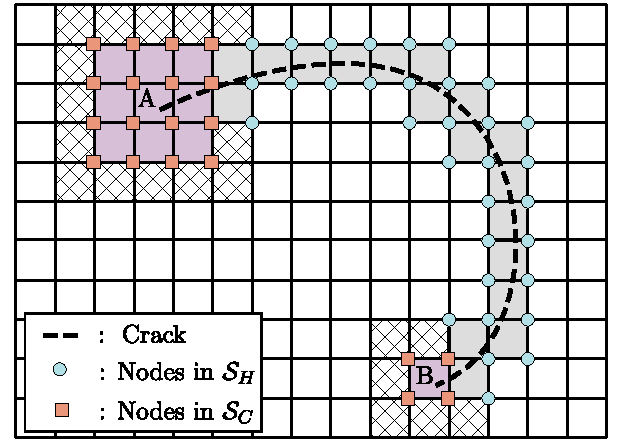
\includegraphics[width=0.55\textwidth]{images/Q6_XFEM.pdf}
    \caption{An arbitrary crack line (dashed line) in a structured mesh with step enriched (light gray) and tip enriched (purple) elements. Nodes in sets $\mathcal{S}_C $ and $\mathcal{S}_H$ are denoted by red squares and blue circles, respectively~\cite{Belytschko.2009}.}
    \label{fig:XFEM}
\end{figure}

\hspace{1em}Although XFEM come with an advantage of simulating a random crack propagation and giving it more freedom for the crack to propagate, this come to the disadvantage and also one of the challenging task
in implementing this model. The challenge lies as the crack propagates to the node, this will give an unstable result, since the distance from the node to crack tip is nearly zero according to the relation of crack tip
relation that proportional to $\sqrt{\frac{1}{r}}$, leading to very large stress contribution. Therefore, the model stability is a highly dependent on the mesh, as decreasing the mesh size is prone for the crack pass through the node.

\section{Damage mechanics}
\hspace{1em}The last approach for modelling fracture and considered one of the reliable model and have wide range usage especially in explicit dynamic application is
damage mechanism. To understand the basic term of damage, let us consider a cylindrical specimen, which posses holes inside the volume. In figure~\ref{fig:DamageSpecimen}, $A_{eff}$ denote as the effective area. Where it stands
for the area that is still capable of holding a stress, which the area is smaller than the area $A_0$ before it was damaged. 

\begin{figure}[H]
    \centering
    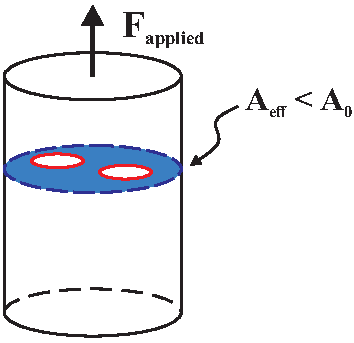
\includegraphics[width=0.4\textwidth]{images/Q7_DamageSpecimen.pdf}
    \caption{Damaged cylindrical specimen shows in red coalescence of void with the applied force.}
    \label{fig:DamageSpecimen}
\end{figure}

\hspace{1em}The relation of the effective and initial area can be written as follows.

\begin{equation}
  A_{eff} = (1-D)A_0
  \label{eq:AreaDamage}
\end{equation}

\hspace{1em}Where D is damage parameter, ranging in between [0, 1]. Therefore, the final effective stress applied in the specimen with damage can be summarized as follows.

\begin{equation}
  \tilde{\sigma} = \frac{F}{A_{eff}} = \frac{F}{(1-D)A_0}
  \label{eq:StressNew}
\end{equation}

\hspace{1em} This will eventually introduce larger value of stress by due to the fact that the area is reduced by the presence of the damage parameter. This damage parameter visualize not only for stress, but also for the effective stiffness as well. As an example, following figure
shows the flow curve, which produced by the author in the 2nd assignment, highlighting the damage area. As it can be seen from the curve, the effective stiffness is gradually decreased as the damage accumulated in higher strain level.

\begin{figure}[H]
    \centering
    \begin{tikzpicture}
        
        %% --- PRIMARY AXIS: STRESS-STRAIN (Bottom & Left) ---
        \begin{axis}[
            scale only axis,
            width=0.85\textwidth,
            height=5cm,
            xlabel={Strain},
            ylabel={Stress in MPa},
            axis y line*=left,
            axis x line*=bottom,
            xmin=-0.004, xmax=0.075,
            ymin=-20, ymax=300,
            grid=major,
            xticklabel style={/pgf/number format/fixed, /pgf/number format/precision=2},
            legend style={at={(0.65,0.7)}, anchor=north west}
        ]
            \addplot[color=black, line width=2pt] 
                table{Visualization/resources/Case1.txt};

            \fill[red, opacity=0.1] (axis cs:0.025, -20) rectangle (axis cs:0.075, 300);
            
            \draw[black, 
                  line width=1pt] (axis cs:-0.004, 0) -- (axis cs:0.075, 0);

            %% Triangle
            \draw[black, 
                  line width=1pt] (axis cs:0.0015, 50) -- (axis cs:0.0015, 250);
            \draw[black, 
                  line width=1pt] (axis cs:0.0005, 50) -- (axis cs:0.0015, 50);

            \node[label={right:E}, inner sep=2.5pt] 
            at (axis cs:0.001, 135) {};

            %% Second Triangle
            \draw[black, 
                  line width=1pt] (axis cs:0.025, 50) -- (axis cs:0.025, 250);
            \draw[black, 
                  line width=1pt] (axis cs:0.024, 50) -- (axis cs:0.025, 50);

            \node[label={right:E}, inner sep=2.5pt] 
            at (axis cs:0.025, 135) {};

            %% Third Triangle

            \draw[black, 
                  line width=1pt] (axis cs:0.035, 0) -- (axis cs:0.043, 100);

            \draw[black, 
                  line width=1pt] (axis cs:0.04, 25) -- (axis cs:0.04, 62);

            \draw[black, 
                  line width=1pt] (axis cs:0.037, 25) -- (axis cs:0.04, 25);

            \node[label={right:(1-D)E}, inner sep=2.5pt] 
            at (axis cs:0.04, 38) {};

            \draw[black, 
                  line width=1pt, 
                  dash pattern=on 5pt off 2pt] (axis cs:0.0238, 0) -- (axis cs:0.025, 285.101);
            
            \node[label={right:Damage State}, circle, fill=black, inner sep=2.5pt] 
            at (axis cs:0.043, 100) {};
            
  
            

            \addlegendentry{Stress-Strain}
            
    
        \end{axis}

        %% --- SECONDARY AXIS: DAMAGE (Top & Right) ---
        \begin{axis}[
            scale only axis,
            width=0.85\textwidth,
            height=5cm,
            % --- ADD TITLE HERE ---
            %title={\textbf{Engineering Stress-Strain and Damage Evolution for Q1 Plate}},
            %title style={yshift=2.5em}, % Moves title up to avoid hitting top X-axis labels
            % ----------------------
            % --- Independent Scales ---
            xmin=-0.04, xmax=0.75,           % Normalized Time or separate X-data
            ymin=-2/30, ymax=1.05,           % Damage (0 to 1)
            axis y line*=right,         % Y-axis on the right
            axis x line*=top,           % X-axis on the top
            xlabel={Time in s},
            ylabel={Damage Variable (D)},
            ylabel style={align=center},
            ylabel style={black},
            xlabel style={black},
            xticklabel style={black},
            yticklabel style={black},
            legend style={at={(0.65,0.6)}, anchor=north west}
        ]
            \addplot[color=black, line width=1.5pt, dashed] 
                table{Visualization/resources/Case1_Damage.txt};

            
            \addlegendentry{Damage Evolution}
        \end{axis}
    \end{tikzpicture}
    \caption{Stiffness degradation, which the effective stiffness value $E_{eff} = (1-D)E$ in the fracture until failure region (red area).}
    \label{fig:StiffnessDegrade}
  \end{figure}

\section{Comparison of the above methods}
\hspace{1em}To distinguish the differences of the discussed three methods in describing fracture, following is the table summarized the difference for the described fracture models.

\begin{table}[h!]
    \centering
    \caption{The difference for each fracture models.}
    \label{tab:FractureDifferences}
    \begin{tabularx}{\textwidth}{l *{7}{>{\centering\arraybackslash}X}}
        \toprule
        Fracture Models / Aspect & Cohesive Zone & XFEM & Damage mechanics \\
        \midrule
        Computational Cost & Moderate (additional criterion between nodes) & Highest (Due to additional DoF) & Lowest (No further DoF addition, only defining the damage criterion) \\
        Predictive Capability & Crack only defines in the designated nodes connection & Crack propagates only in the enriched elements & Damage can occur at any area, as long as the criterion fulfilled \\
        Disadvantage & Crack cannot propagate to other elements due to limitation & Prone to instability due to singularity if the crack propagate to the nodes & Cannot visualize the crack specifically, rather only the damage area  \\
        \bottomrule
    \end{tabularx}
\end{table}

\newpage
\printbibliography

\newpage
\section*{Appendix: Large-Language Models (LLMs) use in this report based on GPT@RUB}


%% ---------------------------------------- %%

\begin{summarybox}{Prompt 1: Outline summary on the evaluation report}
\textbf{Prompt:} You are an expert in fracture mechanics. Can you help me creating a report on following topic summary for my 15 pages report? Here is the topic that I need to write.
\begin{itemize}
    \item Linear Elastic Fracture Mechanics (LFEM)
    \item Elastic-Plastic Fracture Mechanics
    \item Failure hypotheses (critical stress intensity factor, critical energy release rate, J-integral, crack-tip opening displacement)
    \item Crack resistance and R-curve behavior
    \item Cohesive Zone Models
    \item eXtended Finite Element Method (XFEM)
    \item Damage mechanics
    \item Comparison of the above methods
\end{itemize}

Please make the important outlines, which I need to discuss in my report.
\vspace{1em}

\textbf{Response:}

Certainly! Here’s a detailed outline for your 15-page report on the given fracture mechanics topics. This structure ensures logical flow, covers all requested points, and provides subtopics you can expand upon in each section.
\vspace{1em}

\textbf{Title:}

Advanced Topics in Fracture Mechanics: From Linear Elasticity to Damage Modeling
\vspace{1em}
\textbf{Abstract:}

\begin{itemize}
    \item Brief summary of the report’s scope, objectives, and key findings.
\end{itemize}


\textbf{Table of Contents:}

\begin{itemize}
    \item List all main sections and subsections.
\end{itemize}
\end{summarybox}


\newpage
\begin{summarybox}{Prompt 1: Outline summary on the evaluation report}
    
\section*{1. Introduction }
\begin{itemize}
    \item Importance of fracture mechanics in engineering
    \item Historical development and motivation
    \item Overview of report structure
\end{itemize}
\section*{2. Linear Elastic Fracture Mechanics (LEFM)}
\begin{itemize}
    \item Fundamental assumptions (linearity, small-scale yielding)
    \item Stress intensity factor (SIF): Modes I, II, III
    \item Griffith’s criterion and energy balance
    \item Irwin’s modification and practical implications
    \item Applications and limitations
\end{itemize}

\section*{3. Elastic-Plastic Fracture Mechanics (EPFM) }
\begin{itemize}
    \item Need for EPFM: limitations of LEFM
    \item Concepts of plastic zone and crack tip blunting
    \item Key parameters: J-integral, Crack Tip Opening Displacement (CTOD)
    \item Experimental methods for EPFM
    \item Applications and limitations
\end{itemize}
\section*{4. Failure Hypotheses in Fracture Mechanics }
\begin{itemize}
    \item Critical Stress Intensity Factor ($K_{IC}$)
    \begin{itemize}
        \item Definition and measurement
        \item Material toughness
    \end{itemize}
    \item Critical Energy Release Rate ($G_{IC}$)
    \begin{itemize}
        \item Relationship with $K_{IC}$
        \item Energy-based failure criteria
    \end{itemize}
\end{itemize}
\end{summarybox}

\newpage
\begin{summarybox}{Prompt 1: Outline summary on the evaluation report}

\begin{itemize}
    \item $J$-integral
    \begin{itemize}
        \item Path independence
        \item Physical meaning and calculation
    \end{itemize}
    \item Crack Tip Opening Displacement (CTOD)
    \begin{itemize}
        \item Measurement and significance
        \item Relation to ductile fracture
    \end{itemize}
\end{itemize}
\section*{5. Crack Resistance and R-Curve Behavior }
\begin{itemize}
    \item Definition of R-curve
    \item Mechanisms of crack resistance (e.g., toughening, bridging)
    \item Measurement and interpretation of R-curves
    \item Importance in material selection and design
\end{itemize}
\section*{6. Cohesive Zone Models (CZM) }
\begin{itemize}
    \item Concept and historical development
    \item Traction-separation laws
    \item Implementation in numerical simulations
    \item Advantages and limitations
    \item Applications (e.g., interface fracture, ductile tearing)
\end{itemize}
\section*{7. eXtended Finite Element Method (XFEM) }
\begin{itemize}
    \item Motivation for XFEM (limitations of traditional FEM)
    \item Basic principles (enrichment functions, crack representation)
    \item Implementation steps
    \item Applications in fracture analysis
    \item Advantages and challenges
\end{itemize}
\end{summarybox}

\begin{summarybox}{Prompt 1: Outline summary on the evaluation report}
\section*{8. Damage Mechanics }
\begin{itemize}
    \item Introduction to continuum damage mechanics (CDM)
    \item Damage variables and evolution laws
    \item Coupling with fracture mechanics
    \item Applications in predicting failure and life assessment
\end{itemize}

\section*{9. Comparison of Fracture Mechanics Methods }
\begin{itemize}
    \item Summary table of methods (LEFM, EPFM, CZM, XFEM, Damage Mechanics)
    \item Criteria for comparison:
    \begin{itemize}
        \item Applicability (material, loading, geometry)
        \item Accuracy and computational cost
        \item Experimental requirements
        \item Predictive capabilities
    \end{itemize}
    \item Discussion of strengths and weaknesses
    \item Guidelines for method selection
\end{itemize}
\vspace{1em}
\textbf{Tips for writing:}
\vspace{1em}
\begin{itemize}
    \item Use diagrams and figures to illustrate concepts (e.g., SIF, R-curve, CZM).
    \item Include equations where relevant (e.g., Griffith’s criterion, J-integral).
    \item Provide real-world examples or case studies for each method.
    \item Summarize each section with key points.
\end{itemize}
\end{summarybox}

\newpage
\begin{summarybox}{Prompt 2: XFEM singularity}
\textbf{Prompt:} Why does the XFEM will lead to singularity if the crack reach the nodes?
\vspace{1em}

\textbf{Response:}

Great question! Here’s a clear explanation:

Why does XFEM lead to singularity if the crack reaches the nodes?
XFEM (eXtended Finite Element Method) enriches the standard finite element approximation to model cracks without remeshing. It does this by adding special functions to the displacement field:

\begin{itemize}
    \item \textbf{Heaviside function:} to represent displacement jumps across the crack surface.
    \item \textbf{Crack tip enrichment functions:} to capture the singular stress field near the crack tip.
\end{itemize}

\textbf{What happens when the crack reaches a node?}

\begin{itemize}
    \item In XFEM, enrichment functions are applied to nodes whose support is cut by the crack or near the crack tip.
    \item The crack tip enrichment functions are designed to reproduce the singularity in the stress and displacement fields as predicted by LEFM (e.g., $r^{\frac{1}{2}}$
  behavior near the tip).
\end{itemize}

\textbf{If the crack tip coincides exactly with a node:}
\begin{itemize}
    \item The enrichment function becomes singular at that node (e.g., r=0), leading to infinite values in the displacement or stress field.
    \item This is a mathematical singularity, not a physical one, and it causes numerical instability or ill-conditioning in the system of equations.
\end{itemize}

\textbf{Why is this a problem?}
\begin{itemize}
    \item The finite element method relies on evaluating shape functions and their derivatives at nodes.
    \item If the enrichment function is singular at a node, the stiffness matrix entries can become infinite or undefined.
    \item This leads to poor convergence, inaccurate results, or even failure of the solver.
\end{itemize}

\end{summarybox}
\begin{summarybox}{Prompt 2: XFEM singularity}
\textbf{How is this avoided?}
\begin{itemize}
    \item In practice, XFEM implementations ensure that the crack tip does not coincide exactly with a node.
    \item The crack tip is usually placed within an element, not at a node, so the singularity is only approached, not reached.
    \item If the crack tip moves and reaches a node, remeshing or special treatment is required to avoid the singularity.
\end{itemize}

\textbf{Conclusion}

\textbf{XFEM leads to singularity if the crack tip reaches a node because the enrichment functions (especially those modeling the crack tip singularity) become infinite at that point, causing numerical instability.}
To avoid this, cracks are kept within elements, not at nodes, in XFEM simulations.

\vspace{1em}
If you need a more technical explanation or references, let me know!

\end{summarybox}

\begin{summarybox}{Prompt 3: C-Level Displacement}
\textbf{Prompt:} What C level should displacement have in bare minimum in order to not introduce displacement jump?
\vspace{1em}

\textbf{Response:}
In fracture mechanics, \textbf{the regularity (smoothness) of the displacement field} is crucial, especially when modeling cracks. The “C level” refers to the continuity class of a function:

\begin{itemize}
    \item $C^0$: The function is continuous, but its derivatives may not be.
    \item $C^1$: The function and its first derivative are continuous.
    \item $C^2$: The function and its first and second derivatives are continuous.
    \item And so on
\end{itemize}

Displacement Jump and Continuity

A \textbf{displacement jump} occurs when the displacement field is discontinuous 
across a surface (such as a crack). To \textbf{avoid a displacement jump}, the 
displacement field must be at least \textbf{continuous} across the domain, including the crack surface.

\vspace{1em}
\textbf{Bare Minimum Requirement}
\begin{itemize}
    \item Displacement field must be  continuous (i.e., no jump in displacement).
    \item If the displacement field is less than  (i.e., discontinuous), a displacement jump will be present.
\end{itemize}

\textbf{In Practice}
\begin{itemize}
    \item In standard finite element methods (FEM), shape functions are usually $C^0$ continuous, ensuring no displacement jump between elements.
    \item In methods like XFEM (eXtended Finite Element Method), special enrichment functions are used to allow for displacement jumps across cracks, which is necessary for modeling crack opening.
\end{itemize}

\textbf{Conclusion:}

\vspace{1em}

\textbf{The bare minimum C level to avoid introducing a displacement jump is} $C^0$ \textbf{(continuous displacement field)}.

If you want to model cracks with opening (displacement jump), you intentionally use less than $C^0$
  continuity (e.g., in XFEM or cohesive zone models). For standard, uncracked domains, $C^0$
  is required to avoid jumps.

\end{summarybox}


\end{document}

